% Ablation-only section fragment for the DASO paper.
% Required packages in the parent document: graphicx, booktabs, multirow.
% Figure paths are relative to this consolidation directory.

\subsection{Ablation Studies}
\label{sec:ablation}

We conduct all ablations on Llama3.1-8B-Instruct. Unless otherwise noted, we
use the prefill--decode workload with batch size 8, an input length of 2048,
and an output length of 64. We first isolate the components of the latency and
quality predictors, then study the calibration-set size, and finally quantify
the effectiveness of the asynchronous phase-switch runtime.

\paragraph{Latency- and quality-model components.}
Table~\ref{tab:modeling-ablation} reports cumulative ablations of the proposed
predictors. For kernel prediction, we construct a strict generalization split
whose test set contains 4,657 samples from unseen $(N,K)$ shape groups. A
direct data-driven shape fit obtains 14.80\% MAPE. Introducing the
method-specific Roofline prior reduces the error to 10.78\%, demonstrating
that the analytical compute--traffic structure improves extrapolation beyond
the profiled shapes. Modeling the remaining shape-dependent residual further
reduces MAPE to 8.01\%. Thus, both the physical prior and the learned shape
correction contribute to the final kernel predictor.

The refined kernel predictor is fixed in the E2E composition ablation. Simply
summing module and phase costs leaves an 18.17\% policy-level MAPE because it
does not capture non-Linear runtime overheads and systematic composition bias.
The monotonic PAVA mapping reduces this error to 8.30\% while preserving the
latency ordering learned by the underlying model.

For quality prediction, the error is the held-out MAE of real phase-vLLM
$\Delta\mathrm{NLL}$ over 18 policies. Direct local-error aggregation obtains
an MAE of 0.0571. Adding method-, depth-, and module-aware structural factors
reduces it to 0.0468, and further distinguishing prefill and decode reaches
0.0413. The complete model also improves the held-out Spearman correlation
from 0.920 to 0.963, which is important for ranking candidate policies during
constrained optimization.

\begin{table}[t]
\centering
\small
\caption{Modeling ablation on Llama3.1-8B-Instruct. Kernel prediction and E2E
composition report MAPE; quality prediction reports $\Delta$NLL MAE.}
\setlength{\tabcolsep}{5pt}
\resizebox{\columnwidth}{!}{%
\begin{tabular}{ccc}
\toprule
Ablation type & Variant & Error $\downarrow$ \\
\midrule
\multirow{3}{*}{Kernel prediction}
 & Direct fit & 14.80\% \\
 & + Roofline prior & 10.78\% \\
 & + Shape correction & \textbf{8.01\%} \\
\midrule
\multirow{2}{*}{E2E composition}
 & Raw E2E aggregation & 18.17\% \\
 & + Monotonic E2E calibration & \textbf{8.30\%} \\
\midrule
\multirow{3}{*}{Quality prediction}
 & Local aggregation & 0.0571 \\
 & + Structure awareness & 0.0468 \\
 & + Phase awareness & \textbf{0.0413} \\
\bottomrule
\end{tabular}
}
\label{tab:modeling-ablation}
\end{table}

\paragraph{Calibration-set size.}
Figure~\ref{fig:calibration-size-ablation} varies the number of policy-level
NLL measurements while keeping the 18-policy holdout, model structure, and
training procedure fixed. Every subset retains the five dense/uniform anchors,
and we use ten fixed nested subset orders to quantify subset variation. The
median MAE decreases from 0.0614 with five calibration policies to 0.0403 with
45 policies; it then remains between 0.0387 and 0.0408 over the practical
45--64-policy range. In contrast, the median labeling cost grows continuously
from 3.3 to 63.5 GPU-minutes. We therefore use the frozen 54-policy main model
as a practical budget--accuracy operating point; it obtains 0.0413 MAE with a
recorded cost of 48.6 GPU-minutes. The complete 72-policy audit is retained in
the artifact and reaches 0.0340 MAE at 71.4 GPU-minutes; we do not interpret
the truncated paper plot as evidence of strict asymptotic saturation.

\begin{figure}[t]
\centering
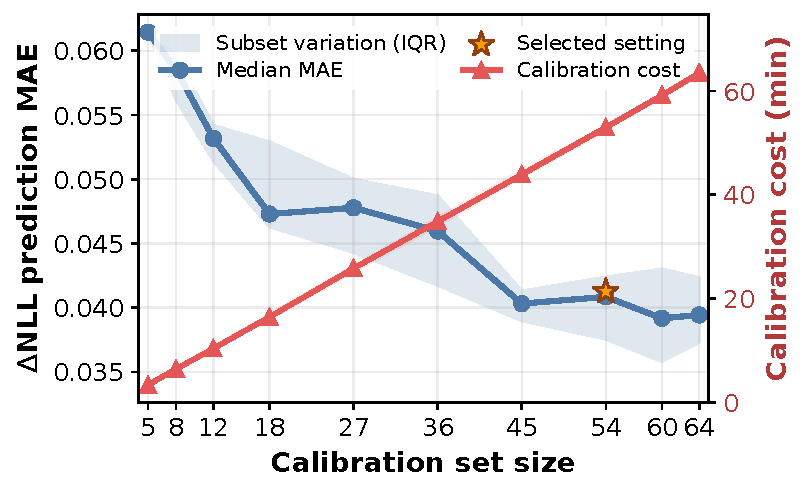
\includegraphics[width=\columnwidth]{figures/calibration_size_sensitivity.pdf}
\caption{Sensitivity to the number of quality-calibration policies. The line
shows the median held-out $\Delta$NLL MAE across ten fixed nested subset orders,
the shaded region shows subset variation, and the secondary axis reports the
measured policy-labeling cost. The star marks the frozen main configuration.}
\label{fig:calibration-size-ablation}
\end{figure}

\paragraph{Asynchronous phase-switch overlap.}
We finally isolate the overlap mechanism in the extended vLLM runtime using
the solved max-speed policy, for which all 128 Linear modules change execution
method between prefill and decode. The synchronous baseline materializes all
decode representations at the phase boundary, whereas our runtime schedules
per-layer transfers on a dedicated copy stream as prefill advances through
the model. Both variants use the same checkpoint, requests, and runtime
configuration and differ only in whether asynchronous prefetch is enabled.

As shown in Table~\ref{tab:runtime-ablation}, asynchronous prefetch reduces the
median E2E latency from 1625.87 to 1521.73 ms across seven paired measurements,
a 6.41\% reduction. More directly, three independent CUDA-event profiles show
that the 128 decode-state materializations contain 354.94 ms of cumulative
transfer work, while only 1.92 ms is exposed as first-use copy stalls on the
compute stream. Therefore, 99.38\% of the transfer work is hidden behind useful
computation. The hidden-work ratio is not expected to equal the E2E speedup,
because concurrent transfers can still contend for PCIe, memory-bandwidth, and
scheduling resources; it instead quantifies how effectively the runtime removes
explicit phase-boundary waiting from the critical path.

\begin{table}[t]
\centering
\small
\caption{Runtime ablation and direct overlap profile on Llama3.1-8B-Instruct.}
\setlength{\tabcolsep}{4pt}
\resizebox{\columnwidth}{!}{%
\begin{tabular}{llc}
\toprule
Scope & Variant or metric & Result \\
\midrule
\multirow{3}{*}{E2E latency}
 & Synchronous boundary copy & 1625.87 ms \\
 & Asynchronous overlap & \textbf{1521.73 ms} \\
 & Relative reduction & \textbf{6.41\%} \\
\midrule
\multirow{3}{*}{CUDA-event profile}
 & Total transfer work & 354.94 ms \\
 & Exposed copy stall & \textbf{1.92 ms} \\
 & Hidden ratio & \textbf{99.38\%} \\
\bottomrule
\end{tabular}
}
\label{tab:runtime-ablation}
\end{table}
